
%(BEGIN_QUESTION)
% Copyright 2010, Tony R. Kuphaldt, released under the Creative Commons Attribution License (v 1.0)
% This means you may do almost anything with this work of mine, so long as you give me proper credit

This distillation tower separates a mixed ``feed'' liquid into two different products called ``distillate'' and ``bottoms'', using liquid level control loops on the top and on the bottom.  The top level control system maintains a constant level of condensed ``distillate'' liquid in the accumulator vessel, while the bottom level control system maintains a constant level of ``bottoms'' liquid in the reboiler vessel:

$$\includegraphics[width=15.5cm]{i03695x01.eps}$$

Suppose an instrument technician mis-calibrates the reboiler level transmitter so that it outputs less signal than it should (representing less liquid level than is actually there).  What effect will this have on the actual liquid level inside the reboiler?  Will the actual liquid level become {\it less} than it should be, {\it more} than it should be, or will it remain exactly {\it as} it should be?

\underbar{file i03695}
%(END_QUESTION)





%(BEGIN_ANSWER)

The actual reboiler liquid level will be {\bf greater} than it should be as a result of the fault.

%(END_ANSWER)





%(BEGIN_NOTES)

{\bf This question is intended for exams only and not worksheets!}.

%(END_NOTES)


